% id: 0113
% book: RPM 중3-2 수학 · 01 삼각비
% section: 유형 15 삼각비의 표를 이용하여 삼각비의 값 구하기
% figure: crop:fig-0113.png
% answer: $104^\circ$
% answer_source: 답지
% variant_level: 0 (원본 전사)
% 이 파일은 build.mjs 가 items.json 에서 만든다. 고칠 때는 items.json 을 고친다.
\smash{\raisebox{1.5mm}{\dmkichul{대표문제}}}
$\sin x=0.7986$, $\cos y=0.6293$일 때, 다음 삼각비의 표를 이용하여 $x+y$의 크기를 구하시오.
\par\smallskip\begin{center}\setlength{\dmfigw}{240.7pt}\ifdim\dmfigw>\linewidth\setlength{\dmfigw}{\linewidth}\fi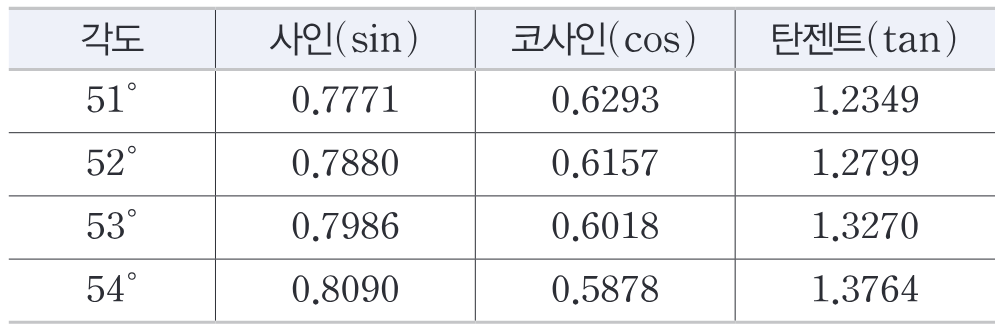
\includegraphics[width=\dmfigw]{figures/fig-0113.png}\end{center}
